\documentclass{article}
\usepackage[margin=1cm, bottom=2cm, portrait, a4paper]{geometry}
\usepackage{fontspec}
\usepackage{amsmath}
\usepackage{indentfirst}
\usepackage{mathtools}
\usepackage{graphicx}

\makeatletter
\newcommand{\xdashleftrightarrow}[2][]{\ext@arrow 3359\leftrightarrowfill@@{#1}{#2}}
\def\rightarrowfill@@{\arrowfill@@\relax\relbar\rightarrow}
\def\leftarrowfill@@{\arrowfill@@\leftarrow\relbar\relax}
\def\leftrightarrowfill@@{\arrowfill@@\leftarrow\relbar\rightarrow}
\def\arrowfill@@#1#2#3#4{%
  $\m@th\thickmuskip0mu\medmuskip\thickmuskip\thinmuskip\thickmuskip
   \relax#4#1
   \xleaders\hbox{$#4#2$}\hfill
   #3$%
}
\makeatother

\title{Информационные технологии. Лекция 11. Мобильная криптография}
\author{Студент группы 2305 Макурин Александр}
\date{15 мая 2023}

\setmainfont[Ligatures=TeX]{Linux Libertine}
\graphicspath{./graphics/}

\begin{document}
\maketitle
Три кита информационной безопасности:
\begin{itemize}
    \item Целостность
    \item Конфиденциальность
    \item Доступность
\end{itemize}

\section*{Система}
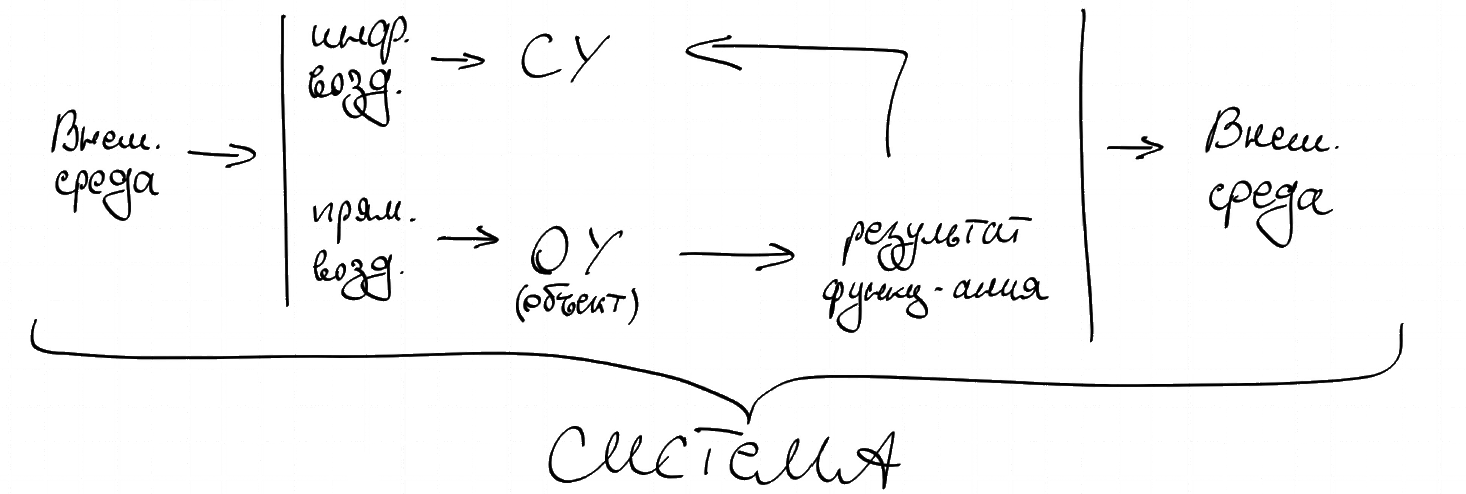
\includegraphics[width=0.7\textwidth]{graphics/pic01.png}

$e_i \xrightarrow{M} e_j$

$M_i \simeq M_j^i$ (информация с $M_i$ на $M_j$) — информация дошла

\begin{enumerate}
    \item $P$ — св-ва $M_i$
          $P_i \neq P_i^j$

          Если хотя бы один не совпадает $\Rightarrow$ нарушена целостность информации.

          $M_i = \cup m_i = \{m_i\}$

          $\{m_i\} \cap \{m_i^j\} \neq \{m_i\}$ — плохо (информация искажена в процессе передачи).
    \item 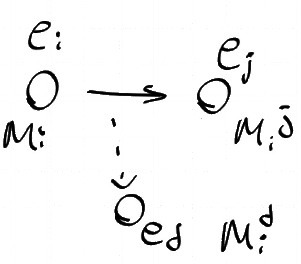
\includegraphics[width=0.3\textwidth]{graphics/pic02.png}

          Если $M^d_i = M_i = M_i^j$ — нарушена конфиденциальность.
\end{enumerate}

Интеллектуальный агент — агент, которй может:
\begin{itemize}
    \item взаимодействовать со средой
    \item обязан иметь целостность
    \item работать без вмешательства из вне
\end{itemize}

В контексте информационной безопасности (ИБ) каналы связи считаются гомогенными.

Модель угроз: \\
Предпосылки к реализации угроз $\rightarrow$ Уязвимость $\rightarrow$ Угроза $\rightarrow$ Нарушитель (элемент МАС).

МАС — мультиагентная система.

Угрозы самообучения — обучение пойдёт не туда. Примеры: Skynet; IBM Watson, которого пытались обучить доказательной медицине, подулючили к интернету, в котором модель нашла словарь ругательств и стала постоянно их использовать.

$X \rightarrow (a: X \rightarrow X_1) \rightarrow (a_1: X_1 \rightarrow X_2) \rightarrow (a_2: X_2 \rightarrow Y) \rightarrow Y$, где $X$ — модель мира в момент $t_i$, $Y$ — план действий $T_{i + 1}$.

$Y = Y_{\text{д}} \cup Y_\text{н}$, где д — допустипый, н — недопустимый.

\subsubsection*{3 способа избавиться от недопустимых:}
\begin{enumerate}
    \item наложить ограничения на $Y$
    \item наложить ограничения на $\{a\}$
    \item наложить ограничения на $X$
\end{enumerate}

\subsubsection*{Направления атак:}
\begin{itemize}
    \item Spoofing (СПАМ)
    \item DOS
    \item Целевые атаки
    \item Атаки на коммуникационные сети
    \item Вирусы
\end{itemize}

Атаки на взаимодействие элементов МАС (ведут к неверному поведению (misbehaviour)):
\begin{itemize}
    \item on-off attack — то атакует, то нет. Невозможно выявить
    \item bad mouth — молчит о другом
    \item ballot stuffing — внесение ложной информации об окружающей среде
\end{itemize}

$Env \xdashleftrightarrow{P_{Env}}e_i \xrightarrow{M} e_j$

$P_{Env} \neq P_{Env}^{e_i}$

$M^{e_i} = f(P_{Env}^{e_i})$

$M^{e_i} \neq \overline{M}(P_{Env})$

$f(P_{Env}^{e_i}) \neq f(P_{Env})$

Проблема потери пакетов на данный момент является относительно решённой.

Функциональная безопасность — защита окружающей среды и системы от самой себя.

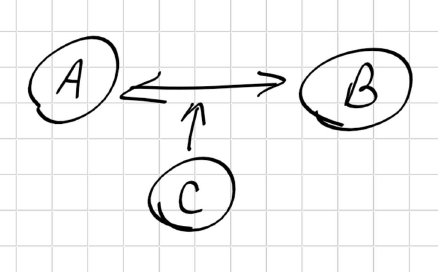
\includegraphics[width=0.5\textwidth]{graphics/pic03.png}

Агент C получил доступ к сообщению от A к B и callback. C может украсть верную информацию или фальсифицировать callback.

$\widetilde{f}(x_i) = y_i$

Вопрос мобильной криптографии — найти такую $f$, что $f(x) = \widetilde{y_i} = E(y_i)$. Здесь $f(x)$ — отправляемая информация, которой владеет A, $\widetilde{y_i}$ — информация, получаемая B (её можно расшифровать), $E(y_i)$ — зашифрованная информация, доступ к которой может получить C.
\end{document}